

\chapter{如何创新} % Introduction chapter suppressed from the table of contents


今天在书店看到这本 ------ 张萌写的 ``人生效率手册''

\hypertarget{ux76eeux5f55ux8282ux9009}{%
\subsubsection{目录节选}\label{ux76eeux5f55ux8282ux9009}}

\begin{itemize}
\tightlist
\item
  目标建立
\item
  时间管理

  \begin{itemize}
  \tightlist
  \item
    有了目标才能开启时间管理之门
  \item
    把大目标分解成小目标,各个击破
  \end{itemize}
\item
  高效学习

  \begin{itemize}
  \tightlist
  \item
    预习,实时学习到最后复习,才是完整的学习过程
  \item
    早起掌控自己的时间,你是时间主人
  \item
    充满正能量,在激励中不断前进
  \end{itemize}
\item
  修炼硬本领
\item
  自我输入与输出

  \begin{itemize}
  \tightlist
  \item
    自我输入输出的渠道,不仅仅是上课听讲
  \item
    孰能生巧后,你才能成为别人的师父
  \item
    写作也是一种输出
  \end{itemize}
\end{itemize}

这书从制定目标开始,然后教你一些提升方法(如时间管理,高效学习等等)。
虽然有很多可参考的技巧,但有很重要一点她没有提到 -
如何驱动人改变以往的习惯?减肥的道理方法,每个人都懂,但为什么还是这么多人体重超标?

例如上一章说到的极限编程里的最佳实践都能很好帮助提升开发质量,现在已经20多年了;\\
质量大师Dr Juran质量手册(Quality Control
Handbook)里面也有很多质量改进的经典,大部分也适用于软件开发,第一版距今也已经50年了;\\
所以不能说没有方法,但为什么很多软件开发团队今天还是有不少质量问题?

锻炼身体或提升编程开发能力也如此。没有明确追求的目标,没有动力,任何好方法都帮不了你。

\hypertarget{ux521bux65b0-creativity}{%
\subsection{创新 Creativity}\label{ux521bux65b0-creativity}}

创新能推动改进,提高生产率。 但创新不局限于软件工程。\\
例如,音乐 - 作曲家都要具备极高的创新能力。\\
Robert FRITZ 回忆到 ``60年代,当我在BOSTON Conservatory
学音乐作曲时,开始思考学的不应仅仅是对位、和音,而是音乐大师的创新过程''
他毕业后继续做音乐创作,一次参加创新专业人士聚会,包括作家、画家、音乐家、建筑师等,他发现这些人在针对本身专业的创作能力都很厉害,但都没有想到用他们的创新能力提升自己的生活。
他便开始举办培训课帮不同背景的人提升创新,让各个行业也可以学什么是创作/创新。几年后,他把创作的重点写成了一本书
(见 Reference 参考)。Robert FRITZ 在他的书中,以贝多芬为例,说明创作并非
problem
solving(解决问题),而是要有一个很高的目标/理想,然后不断地尝试比较,最终达到创作目的。

\hypertarget{ux521bux9020ux7684ux7cbeux795e-spirit-of-creating}{%
\subsection{创造的精神 Spirit of
Creating}\label{ux521bux9020ux7684ux7cbeux795e-spirit-of-creating}}

创作不是由他人驱使,而是出于自身创作的欲望,要做世界上最优秀的作品。作家觉得自己的创作有价值,会用很多的精力进行创作。创作者努力创作,最终希望自己的作品以后有自己的生命力,受后人赞赏。

贝多芬,他对音乐创作的远景 (VISION)------
希望创造前所未有的作品(他觉得当代的作品离这远景还差很远,甚至包括他老师海顿和音乐天才莫扎特的作品)。由这崇高的远景驱动,加上他自身的音乐演奏/作曲能力,不断突破,甚至耳聋也阻挡不了他的创作力(从25岁开始听力减退,到45岁已经完全失聪)。
回顾贝多芬的创作生涯:\\
%\url{文件:Bdf.png}



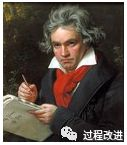
\includegraphics[width=10cm]{Bdf.jpg}\\

\framebox{%
\begin{minipage}[t]{0.97\columnwidth}\raggedright
\textbf{贝多芬} (1770 --
1827)的音乐创新可以说是前无古人后无来者,深深影响后面两世纪的作曲家。\\
我们都熟识他的命运交响曲,其实他从1795年到1827年去世前出版的每一首作品,无论是交响曲、室内乐、歌剧,都是经典。他是完美主义者,例如,田园交响曲(与命运同时出版与首演)的创作时间不少于3年,从他手稿得知,首乐章某主题他修改了不下12次,所以与莫扎特,舒伯特比较,他的``生产率''不算高,平均每年出版5\textasciitilde{}6个作品。

他出版命运、田园交响曲时(1808),已经出版音乐作品十三年,包括23首钢琴奏鸣曲,9首弦乐四重奏。
开始时,他与古典时期的海顿、莫扎特的风格类似,但是到了中期,如命运交响曲、田园交响曲,已经远远超出他前辈和同辈,启蒙音乐家从古典期发展成浪漫期新风格。

晚期的作品(如钢琴曲、弦乐四重奏等),又完全另一套与中前期不同风格。例如,他的Op133
弦乐四重奏 Große Fuge
由于思路远超于当时的水平,不被当时的音乐家接受,觉得作品有问题,有些甚至说他太老,不止聋了,并疯了。但贝多芬依然故我,说``这曲是为未来写的!''

他的音乐创作一直没有停下来,例如,他的最后弦乐四重奏(第16首)Op135在1826年出版。
贝多芬 一生写了32 首 钢琴奏鸣曲 ,
与莫扎特和他老师海顿不同,贝多芬每一首钢琴奏鸣曲虽然都是奏鸣曲式 (sonata
form),但都有独特创新,突破奏鸣曲式,变化万千。\strut
\end{minipage}}

他与其他音乐大师有一个共同的特点就是有把握自己命运,追求个人目标的主动心态,再加上本人的天赋、魄力,而非被动解决每天面对的问题
(Problem solving)。

远景 / 理想 /创意 我们大部分人都有,但为什么只有少数能成为大师?
所有创新都需要经过一个漫长的过程。

%\href{文件:liuct.png}{600px}
\includegraphics[width=20cm]{liuct.jpg}\\

\hypertarget{ux76eeux6807ux600eux6837ux8bbe-ux4ec0ux4e48ux6837ux7684ux76eeux6807ux624dux7b97ux7406ux60f3}{%
\subsection{目标怎样设?
什么样的目标才算理想?}\label{ux76eeux6807ux600eux6837ux8bbe-ux4ec0ux4e48ux6837ux7684ux76eeux6807ux624dux7b97ux7406ux60f3}}

妨碍个人或公司
提升的原因之一是觉得资源越多越好办事,现在很多事做不出来是因为资源不够


在杭州某商务酒店看到十几条写在墙上浙商名言,其中一条这么说:

%\href{文件:mingyant.png}{600px}
\includegraphics[width=13cm]{mingyant.jpg}\\
很多美国企业家也曾经是如此想,企业越大越稳固。但他们没有想到如果收购不能为公司带来增值,反而会使企业更脆弱。
个人要提升也不能这样想--`` 我现在能力 (资源)
不足,等我具备充分条件再说吧。''(如想知多些怎样能做到个人极限,可看附件
个人STRETCH的小建议)

丰田大野耐一 说得好 -- ``容易达成的目标不是好目标''
他对丰田员工设的质量目标是零缺陷!

%\href{文件:mubiaozhungt.png}{600px}
\includegraphics[width=13cm]{mubiaozhungt.jpg}\\
除了要对未来有一个远景 (VISION)
目标外,了解现状同样重要。但很多人`看'不到真正的,只`看'到自己想象的。

\framebox{%
\begin{minipage}[t]{0.97\columnwidth}\raggedright
很多画家不是画自己看到的,而是画他想象中的。一天画家带学生到美国新泽西州(New
Jersey)
写生,他指着远处3建筑物:山上的高层住宅;海边的仓库;河流上流的工厂。他问学生,这些建筑物什么颜色?所有学生都告诉他,住宅是红色、仓库是白色、工厂是橙红色。老师派给每个学生一张卡,卡上有一个小洞,小洞让学生只单独看到每个建筑物的一小部分,然后老师再问,现在你看到的什么颜色?
本来没有回应,有个学生说,所有都是蓝色,跟那些整个背景一样,本来那些建筑看起来都是蓝色。你可以想象当你在一个有雾的天,你看远处的山、河流、长街。因为我们中间有个大气层,空气,大气会反射光线,就是天空的光,会导致山看起来是蓝色、紫色。
所以当学生不被建筑物的影响下看颜色时,他才会看到真正的颜色。这个故事说明了,很多时候我们以为看到的不是一个真正的事实。\strut
\end{minipage}}

当管理者天天面对团队,但没有客观的数据,他不会感觉项目质量有问题。

开发团队大部分的缺陷都是在系统测试才被发现。
软件缺陷,越往后发现,返工量就越大。如果能在前面代码扫描,代码评审,单元测试等预先发现,
便可以大大减少返工工作量。\\
例如:项目两百多个系统测试缺陷
引起的返工量可能占总工作量三成以上,但因没有收集数据,大家都已经习惯了。\\
当企业有客观数据时,跟刚才那些学生看一些远景的真正颜色一样,他才知道真正样貌,这对整个公司的改进很重要,我们不仅仅是要定目标,更重要是要真正了解现状,才能感觉到差距,驱动改进,认知有差距,有动力做提升
-- 改变原来的习惯,开始动起来。

\hypertarget{fritz-ux628aux8fd9ux6539ux53d8ux8fc7ux7a0bux7b80ux5355ux5206ux4e3aux4e09ux6b65}{%
\subsection{FRITZ
把这改变过程简单分为三步}\label{fritz-ux628aux8fd9ux6539ux53d8ux8fc7ux7a0bux7b80ux5355ux5206ux4e3aux4e09ux6b65}}

\begin{enumerate}
\tightlist
\item
  Germination 萌芽
\item
  Assimilation 吸收
\item
  Momentum 动力
\end{enumerate}

萌芽是开始动起来,但我觉得中间的 吸收(Assimilation) 阶段
最关键好比我们学骑单车,学游泳,学帆船,如果可以过了这关键阶段,便可持续变为动力,成为常态。

FRITZ 刚进音乐学院开始跟老师上单簧管课,每周老师会给他练习曲,叫他去练 /
准备。第一周的曲子很难,他吹得不好。他本以为老师会叫他从练这曲子但老师接下来第二周挑选另一首比第一周更难的曲目,他第二周也吹不好一直这样。他连续练了六首越来越难的练习曲

过了六周后老师请他再吹第一周的曲子,他很轻松地便把它吹完,吹得比第一次好多了,也没有什么错误,然后老师要他在吹第二周的曲子结果也类似。作者对
assimilation 阶段 的经验教训:

\hypertarget{ux7ee7ux7eedux4e0bux4e00ux6b65ux662fux5e2eux4f60ux6d88ux5316ux73b0ux5728ux8fd9ux6b65ux7684ux6700ux4f73ux65b9ux6cd5}{%
\subsubsection{继续下一步是帮你消化现在这步的最佳方法。}\label{ux7ee7ux7eedux4e0bux4e00ux6b65ux662fux5e2eux4f60ux6d88ux5316ux73b0ux5728ux8fd9ux6b65ux7684ux6700ux4f73ux65b9ux6cd5}}

One powerful way to assimilate your present step is to move on to your
next step

回顾我开始写分享文章时,
虽然很困难,写不好,但我继续尝试慢慢变成习惯。起初只是一些零散的笔记,后面逐渐有主思路,有连贯性。如果可以从远景(vision),经过萌芽,吸收,便可以变成动力(momentum),
成为新的习惯。

\hypertarget{ux5fc3ux4ebaux5408ux4e00}{%
\subsubsection{心人合一}\label{ux5fc3ux4ebaux5408ux4e00}}

要改变以往的习惯(解冰),促进创新与提升,人体也要配合起来:

\framebox{%
\begin{minipage}[t]{0.97\columnwidth}\raggedright
Tips个人解冰 

我爱人是公立医院的物理治疗师,他知道运动对人体健康很重要,他常常提醒我每天要起码半个小时的带氧运动,但我长期出差,一年住商务酒店的时间不少于10个月。开始的时候,因早上要9点前到达客户现场,时间不够,
只可以隔几天早上15分钟 跑跑步,跳跳绳。最多15分钟
然后逐步把跑步的距离目标定高一点,比如酒店附近的一个地标,来回距离有2公里,现在我每天早上基本可以达到每天半小时的运动量。人的生理状态和心理状态是相关的。所以开始天天做运动,是个人解冰的好开始。\strut
\end{minipage}}


\hypertarget{references}{%
\section{References}\label{references}}

1. Robert FRITZ, The path of least resistance for Managers\\
